\documentclass[colorlinks]{thesis-kando}
\usepackage[T1]{fontenc}
\PassOptionsToPackage{defaults=hu-min}{magyar.ldf}
\usepackage[magyar]{babel}
\usepackage{graphicx,amsmath,amssymb,amsthm,hulipsum,bussproofs,hyperref,titlesec}
\usepackage{listings,xcolor,rotating,booktabs,fancyvrb}
\footnotestyle{rule=fourth}
\DeclareMathOperator{\tg}{tg}
\newtheorem{tetel}{Tétel}[chapter]
\newtheorem{lemma}[tetel]{Lemma}
\theoremstyle{definition}
\newtheorem{definicio}[tetel]{Definíció}
\newtheorem{feladat}[tetel]{Feladat}
\theoremstyle{remark}
\newtheorem{megjegyzes}[tetel]{Megjegyzés}
\newtheorem*{megoldas}{Megoldás}
\usepackage[normalem]{ulem}
\usepackage[linguistics]{forest}
\useunder{\uline}{\ul}{}
\usepackage{stackengine,scalerel}
\usepackage{pdfpages}
\setcounter{secnumdepth}{3}
\def\tang{\ThisStyle{\abovebaseline[0pt]{\scalebox{-1}{$\SavedStyle\perp$}}}}

\begin{document}

\institute{Informatika és távközlés ágazat}
\title{HealthBro}
\author{Pocsai Gábor\\Ludvig Péter Dániel\\Szilágyi Jorgosz Máté\\Szoftverfejlesztő és -tesztelő szak}
\supervisor{Németh Bence\\oktató}
\city{Miskolc}
\date{2025}
\maketitle
\tableofcontents

\chapter*{Bevezetés}
\addcontentsline{toc}{chapter}{Bevezetés}
A csapatunk neve Nagy Uncia, amely egy három fős, magas szintű szakértelemmel rendelkező fejlesztői csapat, és célunk egy innovatív edzést követő webalkalmazás megtervezése és fejlesztése, amely lehetőséget biztosít a felhasználók számára az edzésprogramjaik nyomon követésére, dokumentálására és elemzésére.
\newline
A csapatunk munkáját Pocsai Gábor irányítja, aki scrum master szerepét tölti be, és felelős az alkalmazás backend fejlesztéséért, az összes kapcsolódó dokumentáció elkészítéséért és karbantartásáért, valamint a projekt menedzsment és verziókezelési feladatok koordinálásáért, beleértve a Trello táblák naprakészen tartását és a Git rendszer hatékony kezelését.
\newline
A product owner szerepét Szilágyi Jorgosz Máté tölti be, aki az alkalmazás adatbázisának tervezéséért és folyamatos karbantartásáért felelős, biztosítva az adatbázis-struktúra és a projekt igényeinek összhangját. Ő felügyeli az adatbázis fejlesztését, valamint annak integrálását az alkalmazás üzleti logikájával.
\newline
A csapat harmadik fejlesztői tagja, Ludvig Péter Dániel, a frontend fejlesztéséért felelős, aki a felhasználói felület kialakításáért, optimalizálásáért és reszponzivitásáért, valamint a felhasználói élmény javításáért dolgozik, biztosítva, hogy az alkalmazás minden platformon és eszközön optimálisan működjön.
\newline
Bár mindhárom csapattagnak különböző szerepei vannak, minden egyes tag aktívan részt vesz az alkalmazás fejlesztésének minden aspektusában, így biztosítva, hogy a backend, frontend és adatbázis integrációja zökkenőmentes és harmonikus legyen. Az összes fejlesztési folyamat során a csapat folyamatosan együttműködik, hogy a projekt sikeres és magas minőségű végeredményhez vezessen.
\newline
A Nagy Uncia csapat tagjai elkötelezettek a folyamatos kommunikáció és kollaboráció mellett, figyelve arra, hogy az alkalmazás minden komponense összhangban működjön, és a felhasználók számára optimális élményt biztosítson.




\chapter{Technológiák}

\section{Relációs Adatbázis}

A lehető legjobb technológiákat választottuk a programunk elkészítéséhez ezért ezekre jutottunk: 


A relációs adatbáziskezelő rendszerek (RDBMS) olyan programok, amelyek lehetővé teszik az adatok strukturált tárolását és kezelését. Az alapelv az, hogy az adatokat táblák formájában szervezzük, ahol a táblák sorokból és oszlopokból állnak. Minden sor egy egyedi rekordot képvisel, míg az oszlopok az adat típusát határozzák meg (például név, kor, cím).

Az RDBMS lehetővé teszi, hogy az adatok között kapcsolatok létesüljenek. Például egy "Diákok" táblában lehetnek olyan adatok, mint a diák neve, az osztálya és az azonosítója, míg egy "Tanárok" táblában a tanárok neve, tantárgya és azonosítója található. 
\newline
Az RDBMS használata számos előnnyel jár, például:

\begin{itemize}
	\item Adatintegritás: Az adatok konzisztenciája és megbízhatósága.
	\item Adatkezelés: Könnyű adatkeresés, frissítés és törlés.
	\item Könnyű bővíthetőség: Új táblák és kapcsolatok egyszerűen hozzáadhatók.
\end{itemize}
\begin{figure}[h]
	\centering
	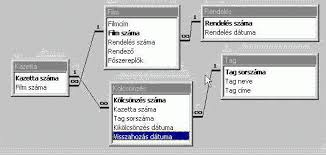
\includegraphics[width=0.5\textwidth]{figures/relacio.jpg}
	\caption{Relációs Adatbázis}
	\label{fig:kep1}
\end{figure}

\section{MySQL és PHPMyAdmin}
Az alkalmazás adatbázis-kezelésére MySQL relációs adatbázis-kezelő rendszert használunk. A MySQL egy széles körben elterjedt, nyílt forráskódú adatbázis-megoldás, amely kiváló teljesítményt, megbízhatóságot és skálázhatóságot biztosít. Lehetővé teszi strukturált adat tárolását és kezelését, támogatja a tranzakciókat, az ACID követelményeket, valamint különböző adattípusokat és relációs kapcsolatokat (pl. one-to-many, many-to-many). Az alkalmazásban a MySQL az Entity Framework Core ORM-mel együttműködve biztosítja a háttérben futó adatbázis-műveletek megbízható végrehajtását.
\newline
Az adatbázis adminisztrációs feladatait a phpMyAdmin webes felületen keresztül végezzük. A phpMyAdmin egy könnyen kezelhető, böngészőalapú eszköz, amely lehetővé teszi a MySQL adatbázis vizuális kezelését. Segítségével egyszerűen hajthatunk végre SQL lekérdezéseket, hozhatunk létre vagy módosíthatunk adatbázisokat, táblákat, nézeteket, kulcsokat, jogosultságokat, illetve végezhetünk adatmentést és visszaállítást is.
\newline
A phpMyAdmin használata megkönnyíti az adatbázis fejlesztési és karbantartási folyamatait, gyors hozzáférést biztosít az adatokhoz, így hatékony támogatást nyújt a fejlesztés és tesztelés során.

\section{React}
A React egy JavaScript alapú könyvtár, amelyet a felhasználói felületek (UI) fejlesztésére használnak, és lehetővé teszi a dinamikus, interaktív webalkalmazások könnyű és hatékony építését.A React legfontosabb jellemzője, hogy a komponens-alapú megközelítéssel segít a UI-k részletekbe menő szervezésében, és a Virtual DOM használatával gyorsítja az alkalmazások renderelését.
Miért is jó a React? Itt felsorolok pár előnyt ami megkönnyíti a munkánkat:
\begin{itemize}
	\item A React-ben a komponenseket más komponensekben is felhasználhatjuk. Ha például a fenti HelloWorld komponenst szeretnénk egy másik komponensben megjeleníteni, ezt így tehetjük meg:

	
	\item Állapotkezelés (State)
	A React egyik legfontosabb funkciója az állapotkezelés. Egy komponens állapota (state) meghatározza, hogy milyen adatokat jelenít meg a felhasználói felület, és a komponens állapotának változása automatikusan frissíti a UI-t.
	
	\item Állapot a useState Hook-kal
	A useState hook segítségével hozhatunk létre állapotot funkcionális komponensekben. Az alábbi példa egy számlálót valósít meg, amely minden kattintásra növekszik.
	A fenti kódban a count a számláló aktuális értéke, amelyet a useState hook inicializál 0-val. A setCount függvény frissíti az állapotot, és újra rendereli a komponenst, ha a felhasználó rákattint a gombra.
	
	\item Állapot több érték kezelésével
	Ha a komponensnek több állapota van, akkor több useState hook-ot is használhatunk, vagy objektumokat, tömböket tárolhatunk az állapotban.
		Itt egy todo lista komponens látható, amelyben minden egyes feladat rendelkezik egy "befejezett" állapottal. A toggleTodo függvény segítségével a feladatok állapota változtatható, és a UI automatikusan frissül.
	
	\item Események és Interakciók
	A React lehetővé teszi az események, például kattintások vagy űrlap beküldések kezelését, az állapot és a renderelés frissítésével.
	
	\item Eseménykezelők használata
	A következő példában egy gomb kattintásra történő eseménykezelőt hozunk létre, amely növeli a számlálót:
	\item Props (Tulajdonságok) Használata
	A props segítségével adatokat adhatunk át egy komponensnek, amelyeket az komponens belső működése során felhasználhat.
\end{itemize}
Összességében a React egy erőteljes és rugalmas eszköz, amely segíti a modern webalkalmazások fejlesztését, miközben egyszerűsíti a kódot és javítja az alkalmazások sebességét.

\section{Entity Framework}
Az alkalmazás adatkezeléséhez a Microsoft Entity Framework Core technológiát használjuk, amely egy modern, nyílt forráskódú objektum-relációs leképezést (ORM) biztosító keretrendszer a .NET platformhoz. Az Entity Framework lehetővé teszi, hogy az adatbázis műveleteket közvetlenül C\# objektumokon keresztül végezzük, anélkül hogy közvetlenül SQL lekérdezéseket kellene írnunk.
\newline
A projektben a Database First megközelítést alkalmazzuk, amely során a már meglévő relációs adatbázis alapján generáljuk le az alkalmazásban használt adatmodell osztályokat és DbContext osztályt. Ez lehetővé teszi, hogy a meglévő adatbázis-struktúrával gyorsan és hatékonyan integrálódjunk, minimalizálva a kézi adatmodell-karbantartás szükségességét.
\newline
Az Entity Framework Core támogatja a LINQ alapú lekérdezéseket, amelyek lehetővé teszik, hogy típusbiztos, könnyen olvasható és karbantartható lekérdezéseket írjunk az adatbázisban tárolt adatokra. Emellett támogatja több különböző relációs adatbázis-kezelő rendszert (pl. SQL Server, PostgreSQL, MySQL), biztosítva a rugalmasságot.
\newline
A Database First megközelítés segítségével az adatbázisban bekövetkező változások egyszerűen követhetők és frissíthetők az alkalmazásban a modell újragenerálásával, így garantálva, hogy mindig naprakész és konzisztens kapcsolat legyen az adatbázis és az alkalmazás között.
\newline
Az Entity Framework használata nagyban hozzájárul a fejlesztési folyamat gyorsításához, az adatkezelési hibák minimalizálásához, és átláthatóbbá teszi az adatbázis-kezelés logikáját.

\section{Swashbuckle}
Az alkalmazás API dokumentációját a Swashbuckle.AspNetCore csomag segítségével valósítjuk meg. A Swashbuckle egy népszerű nyílt forráskódú eszköz, amely automatikusan generál Swagger/OpenAPI dokumentációt az ASP.NET Core Web API projekthez. Lehetővé teszi, hogy az API végpontok részletes leírása, bemeneti paraméterei, válaszai, valamint az esetleges hitelesítési követelmények egy jól strukturált, gépileg olvasható formában legyenek elérhetők.
\newline
Ezen kívül a Swashbuckle integrálja a Swagger UI-t is, amely egy interaktív webes felületet biztosít a fejlesztők és tesztelők számára. Ennek segítségével valós időben kipróbálhatóak és tesztelhetőek az API végpontjai közvetlenül a böngészőből, anélkül hogy külön eszközökre lenne szükség.
\newline
Az alkalmazás konfigurációjában testre szabottan beállításra kerültek az API metaadatai (pl. név, verzió, leírás). 
\newline
A Swashbuckle használata jelentősen megkönnyíti a külső rendszerek fejlesztőinek az API-val történő integrációt, mivel naprakész, pontos és könnyen hozzáférhető dokumentáció áll rendelkezésükre.

\chapter{Bevezetés}
\section{Dokumentum célja}
A dokumentáció célja, hogy részletesen bemutassa a HealthBro weboldal használatát, segítse a felhasználókat az edzések nyomon követésében és a funkciók megértésében.

\section{Használt terminológia}
\begin{itemize}
	\item \textbf{Felhasználónév}:
	\item \textbf{Jelszó}:
	\item \textbf{Email}:
	\item \textbf{Edzésterv}: 
	\item \textbf{Gyakorlat}:
	\item \textbf{Széria}:
	\item \textbf{Súly}:
	\item \textbf{Ismétlés}:
\end{itemize}

\chapter{A rendszer bemutatása}
\section{Áttekintés}
A HealthBro egy online platform, amely lehetővé teszi a felhasználók számára edzéseik nyomon követését, testreszabott edzésprogramok készítését, valamint a fejlődésük monitorozását.

\section{Funkciók rövid ismertetése}
\begin{itemize}
	\item \textbf{Edzések naplózása}: A felhasználók rögzíthetik az elvégzett edzéseket, ismétléseket, súlyokat stb.
	\item \textbf{Célok beállítása}: A felhasználók célokat tűzhetnek ki, mint például izomnövelés, fogyás, vagy állóképesség javítása.
	\item \textbf{Haladás nyomon követése}: Statisztikák és grafikonok a fejlődés megjelenítésére.
\end{itemize}

\section{Rendszerkövetelmények}
\begin{itemize}
	\item Web böngésző (Google Chrome, Mozilla Firefox, stb.)
	\item Internetkapcsolat
	\item Felhasználói fiók a HealthBro weboldalon
\end{itemize}


\section{Weboldal elérési folyamat}
\begin{enumerate}
	\item Nyisd meg a HealthBro weboldalt a böngészőben.
	\item Regisztrálj vagy jelentkezz be a fiókoddal.
	\item Az oldal automatikusan elérhetővé válik minden eszközön, nem szükséges további telepítés.
\end{enumerate}

\chapter{Felhasználói útmutató}
\section{Első lépések}
\subsection{Főoldal}
\fbox{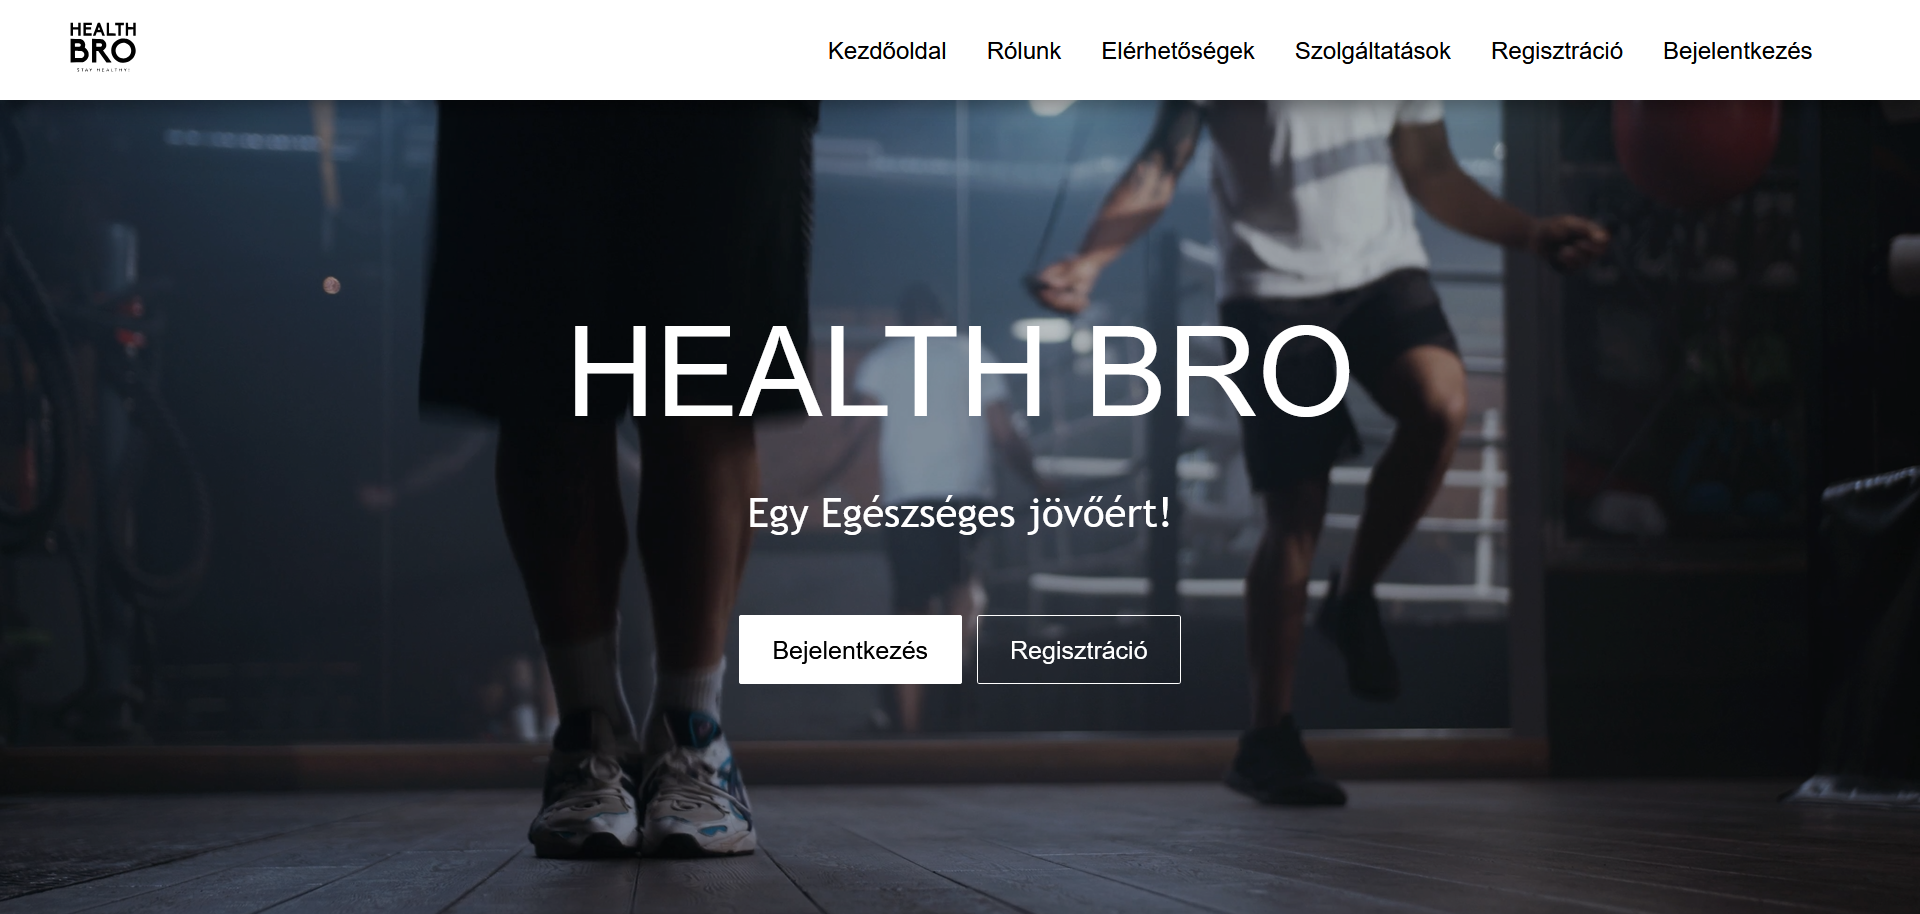
\includegraphics[width=1\textwidth]{figures/homepage.png}\\[0.5cm]}
A weboldalra érkezve, amelyet az alábbi webcímen érhetünk el: healthbro.com, elénk tárul a weboldalunk a healthbro főoldala a “Kezdőlap”. Ezen az oldalon találhatóak a továbbiak is: “Rólunk”, “Elérhetőségek”, “Szolgáltatások”, “Regisztráció” valamint a “Bejelentkezés”.

\subsection{Rólunk oldal}
\fbox{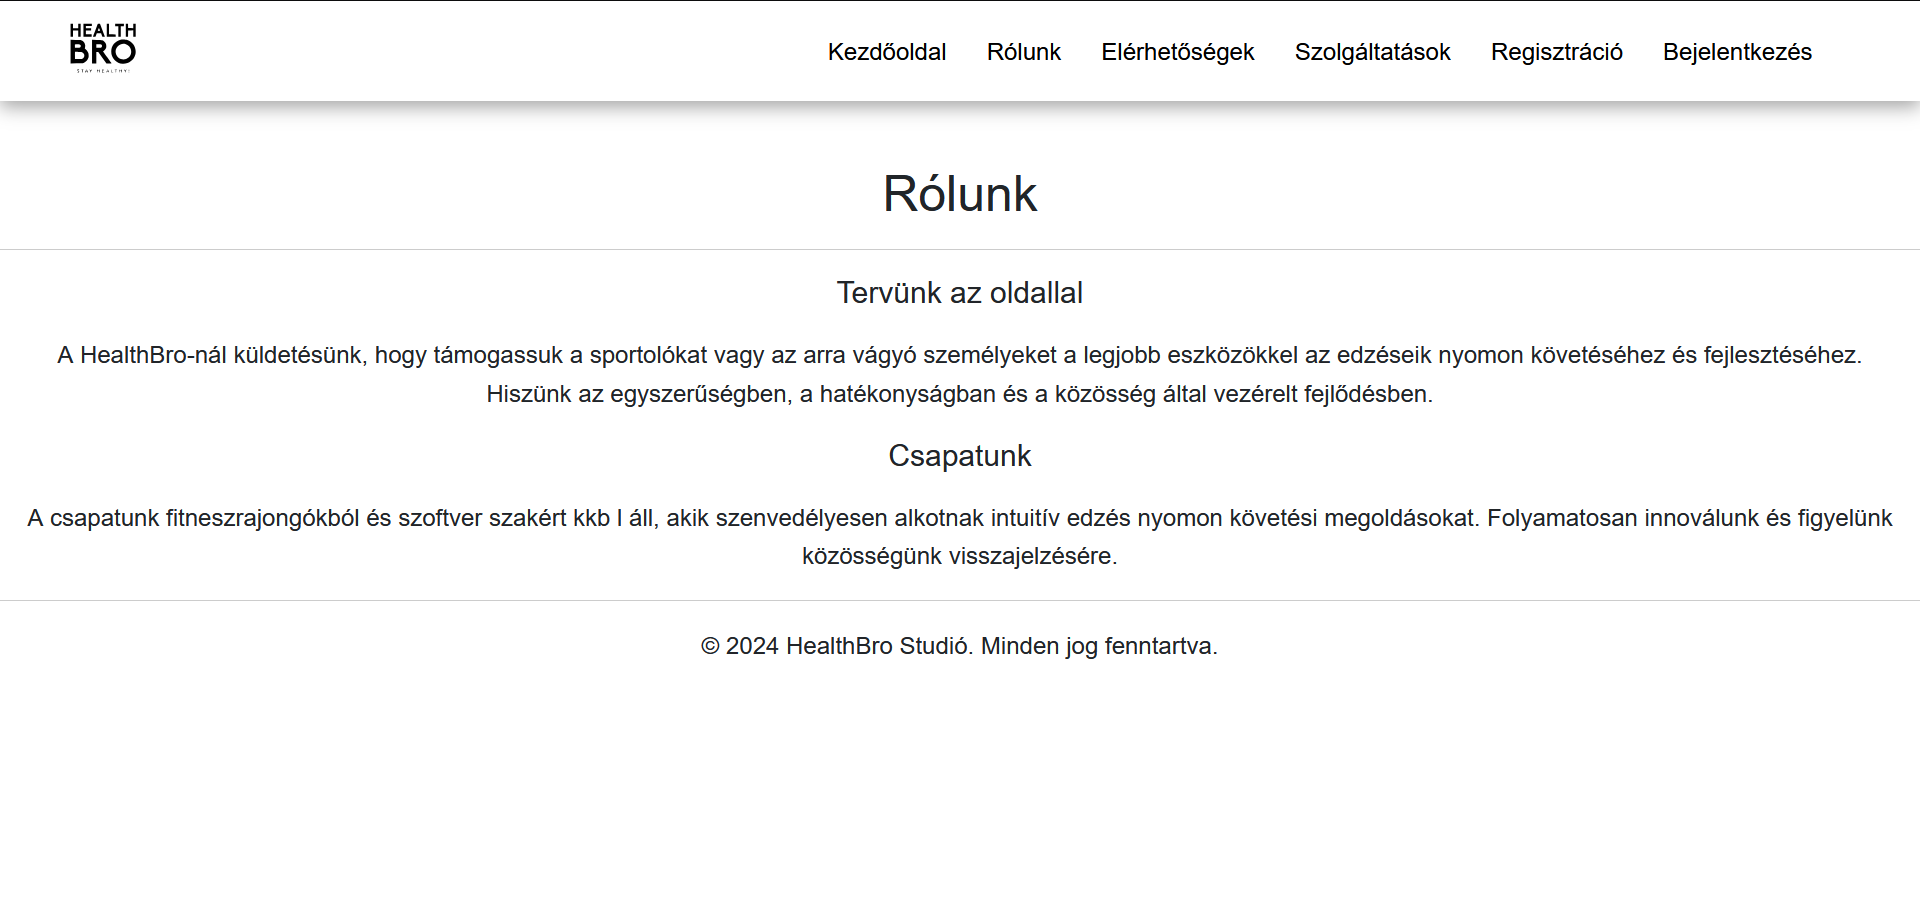
\includegraphics[width=1\textwidth]{figures/rolunk.png}\\[0.5cm]}
A Rólunk menüpontra kattintva láthatóvá válik a csapatunk által alkotott kép, amiben röviden bemutatjuk a csapatunk valamint az oldal terv leírását és annak egyéb terveit a jövőre nézve.

\subsection{Elérhetőségek oldal}
\fbox{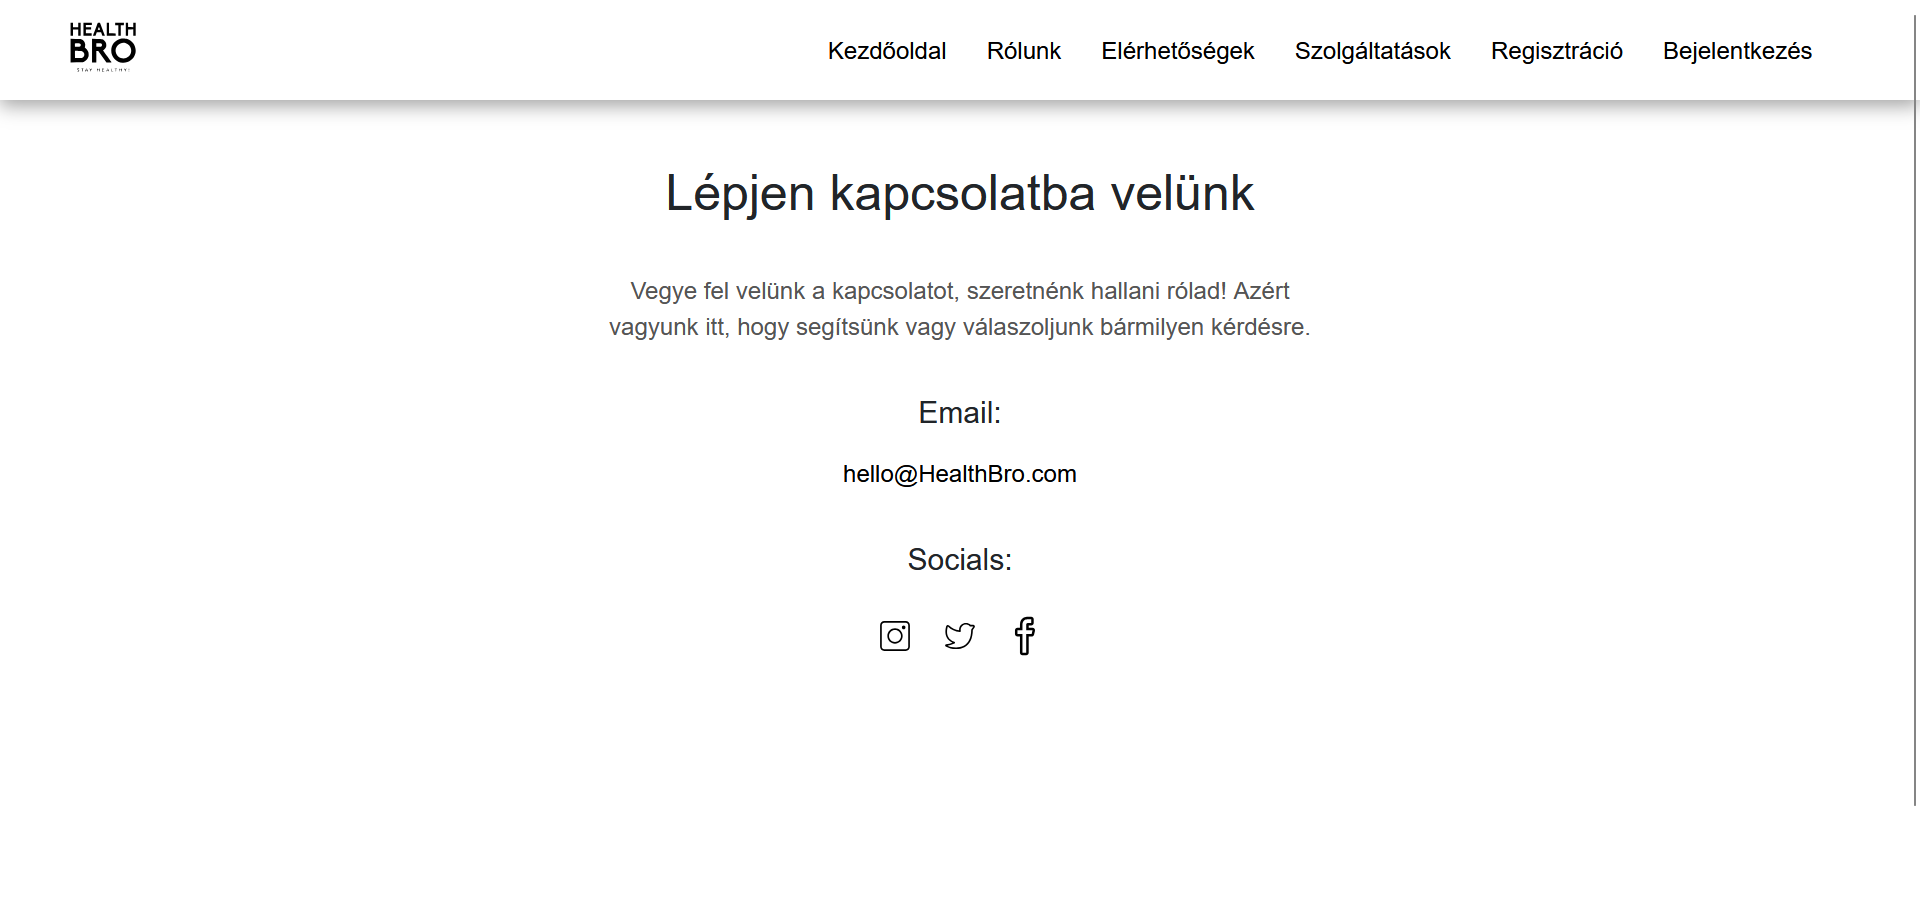
\includegraphics[width=1\textwidth]{figures/kapcsolat.png}\\[0.5cm]}
Az Elérhetőségek menüpontra kattintva a weboldalunk a Healthbro elérhetőségeit.
Az emailen keresztül érhetjük el a supportot, így írhatunk emailt a weboldal fejlesztőinek ha bármi hibát találtunk az oldalon, vagy valami problémánk adódott.
A Socials alatt találhatóak a médiaplatformjaink, ahol képek vagy videók találhatóak az oldalról, bemutató videók vagy átlagos mindennapi média tartalmak, postok. 

\subsection{Szolgáltatások oldal}
\fbox{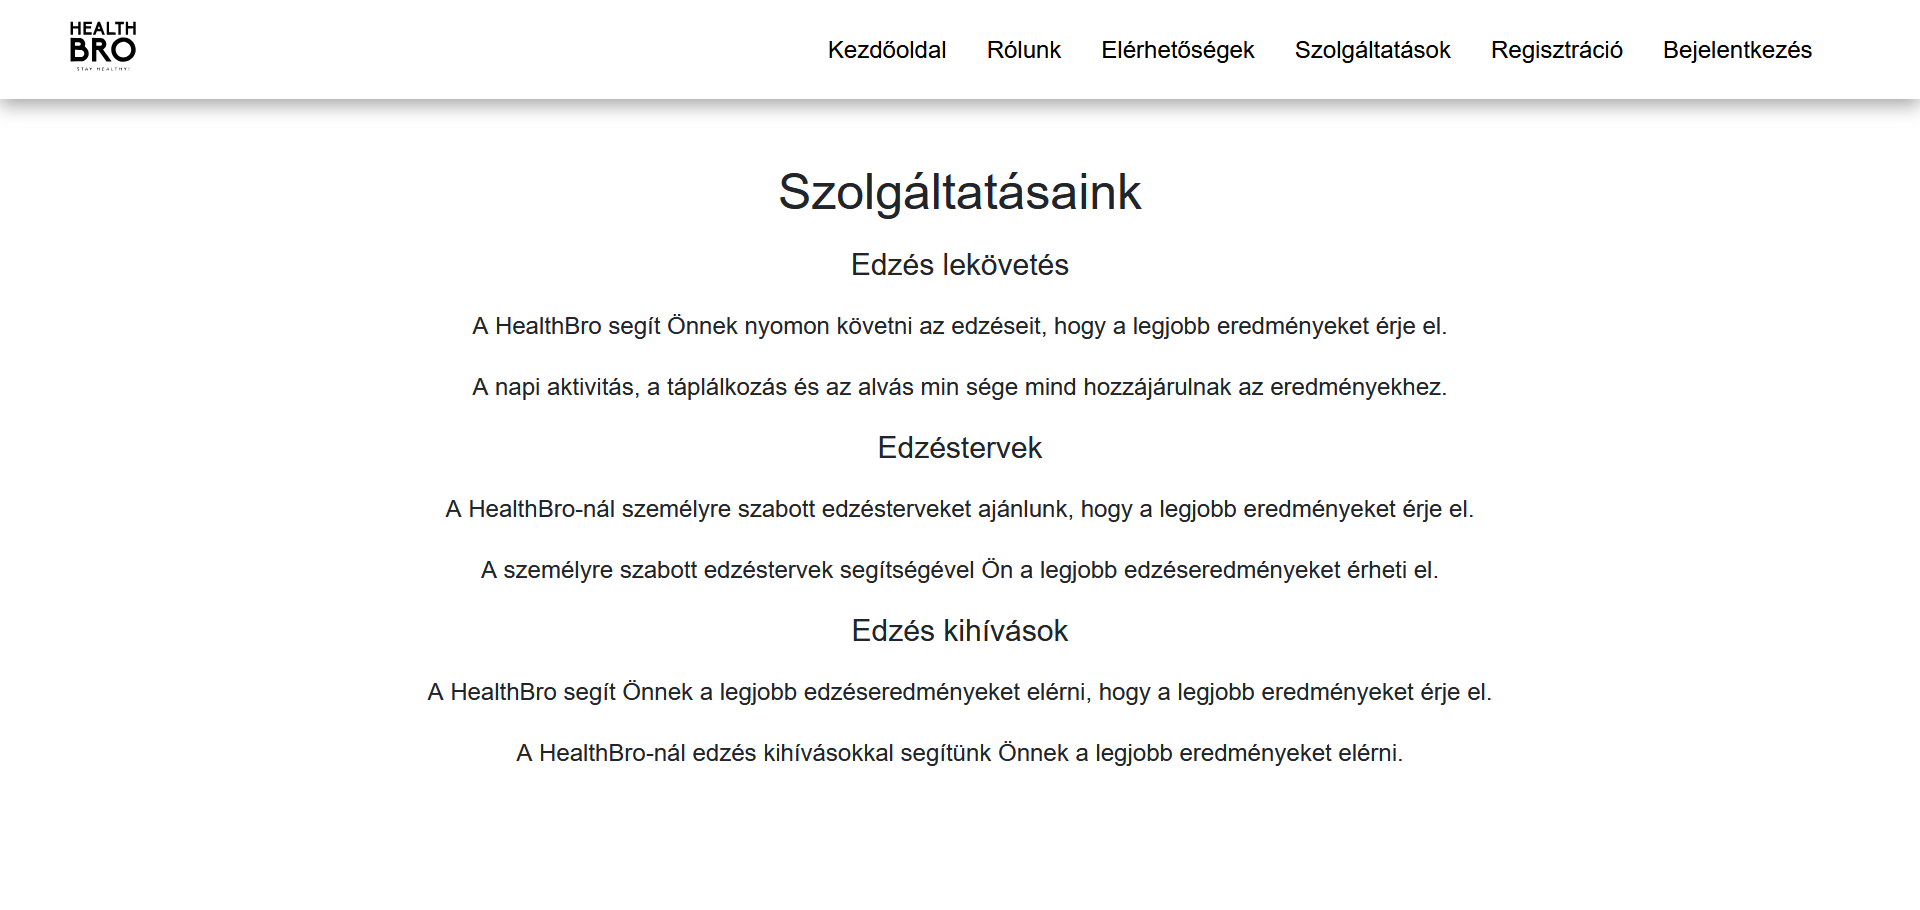
\includegraphics[width=1\textwidth]{figures/szolgaltatasaink.png}\\[0.5cm]}
A Szolgáltatások menüpontra kattintva láthatjuk a weboldal által nyújtott szolgáltatásosainkat, rövid összefoglalók arról, hogy hogyan tudjuk az oldal főbb funkcióit használni vagy hogy hogyan érdemes azt.

\subsection{Regisztráció oldal}
\fbox{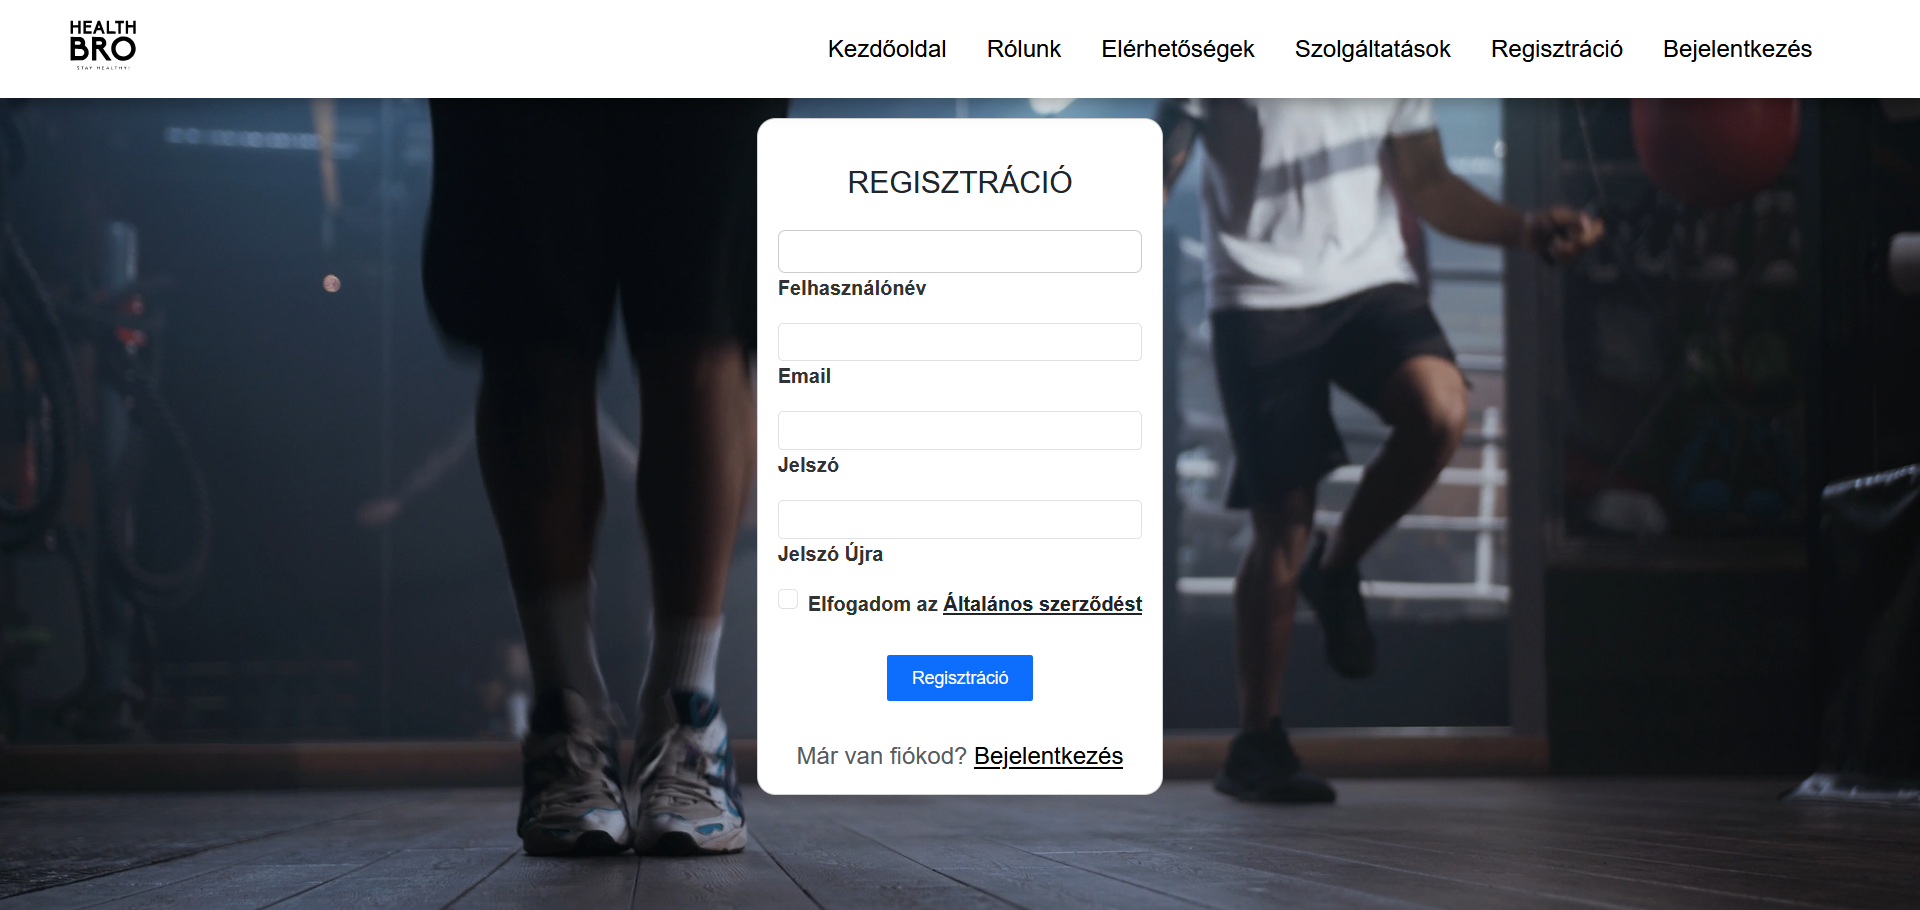
\includegraphics[width=1\textwidth]{figures/regisztracio.png}\\[0.5cm]}
\begin{itemize}
\item A Regisztráció menüpontra kattintva láthatjuk a regisztrációs felületet ahol hamarsoan meg is kezdhetük a saját felhasználónk létrehozását.
Erre szükség lesz az alábbiakra:
\item Felhasználónév (érdemes olyan felhasználónevet használni amit valamely szinten kötődik személyiségünkhöz ezzel elkerülve azt, hogy elfelejtsük).
\item Email (adjuk meg a már létrehozott emailünk valamelyikét, amit gyakran használunk)
\item Jelszó (olyan jelszót válasszunk amit biztosan nem fogunk elfelejteni a jövőben)
\item Jelszó újra (ebben a mezőben meg kell adjuk ugyan azt a jelszót amit az előbbiekben beírtunk, ezzel megerősítve, hogy biztosan nem gépeltük el az először kigondolt jelszónkat)
\item Majd pipáljuk be a kis kockát, hogy elfogadjuk a weboldal szerződését azzal, hogy regisztráljuk új felhasználónkat.
\end{itemize}
Az utolsó pontban viszont átléphetünk a Bejelentkezés oldalra ha már van felhasználói fiókunk létrehozva, ezt megtehetjük a Bejelentkezés feliratra kattintva.

\subsection{Bejelentkezés oldal}
\fbox{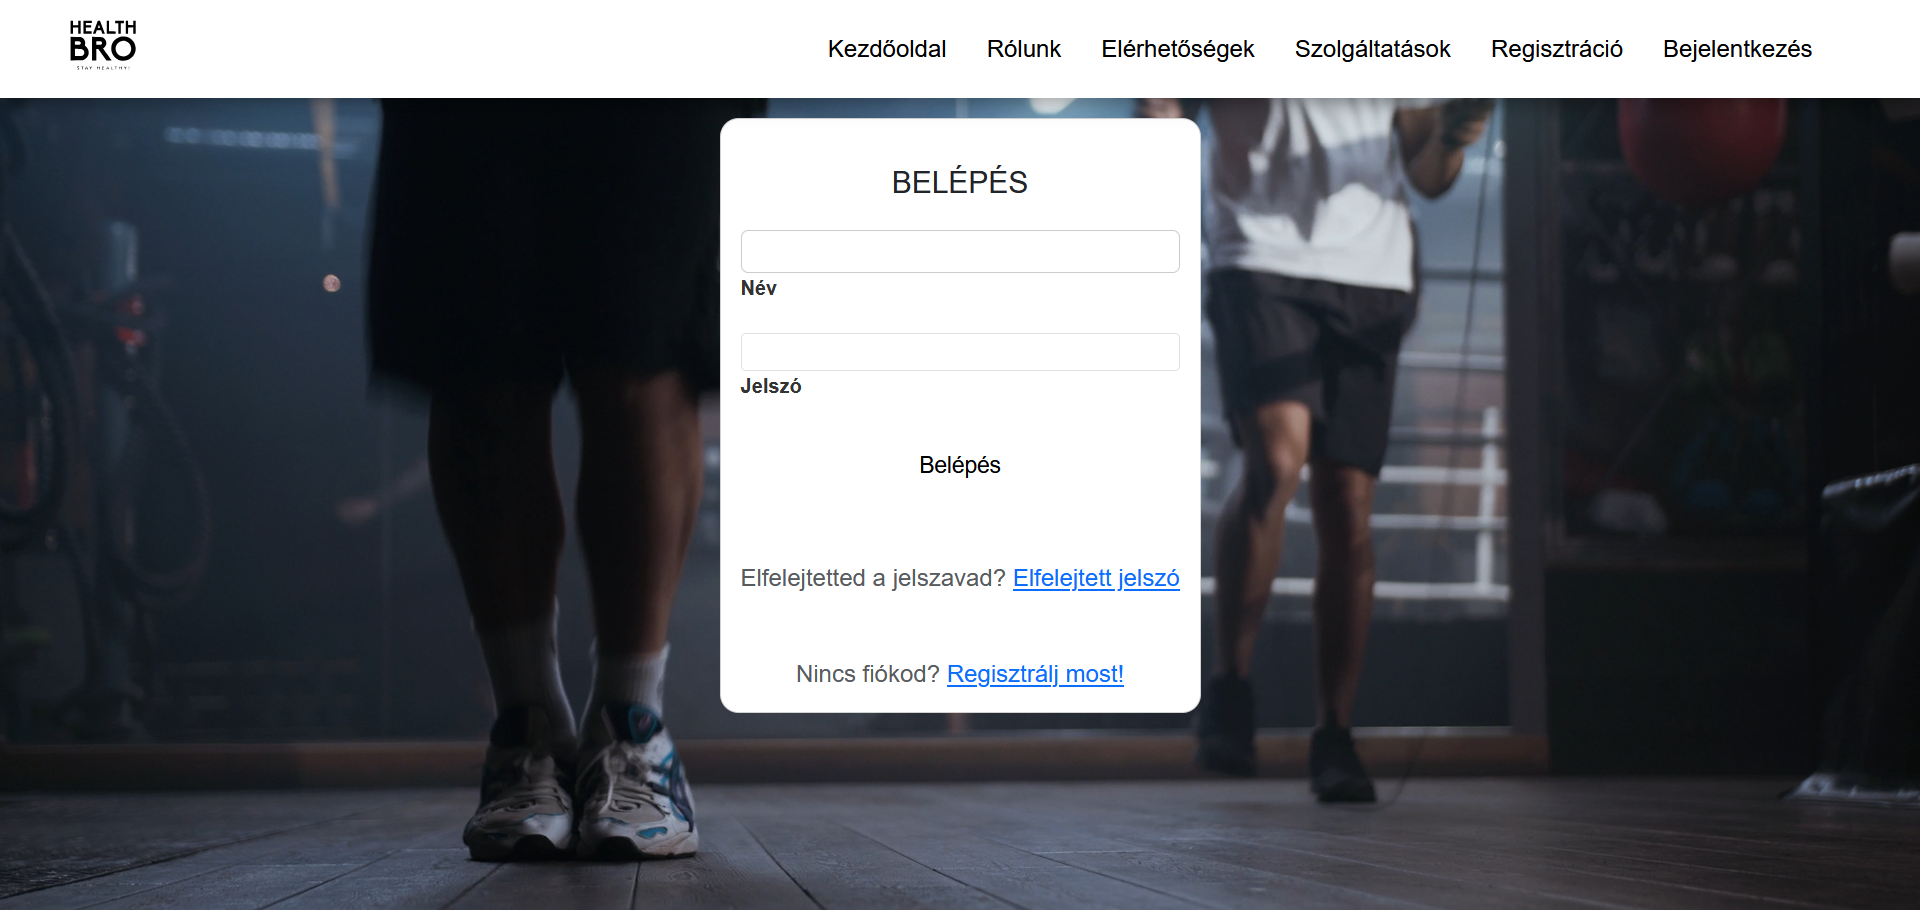
\includegraphics[width=1\textwidth]{figures/belepes.png}\\[0.5cm]}
Ha már előre van létrehozva felhasználói fiókunk, akkor meg is kezdhetjük a bejelentkezést az alábbi mezőket kitöltve:
\begin{itemize}
\item Felhasználónév (már meglévő felhasználónkhoz tartozó felhasználónév)
\item Jelszó (már meglévő felhasználónkhoz tartozó jelszó)
\end{itemize}
Amint ezzel megvagyunk a Belépés gombra kattintva ha helyesen töltöttük ki a 2 mezőt és létezik a felhasználónk, akkor átfog dobni a bejelentkezett főoldalra.
Abban az esetben ha a bejelentkezünk nem sikerül, akkor van lehetőségünk vissza állítani a jelszónkat. Az Elfelejtett jelszó szövegre kattintva átirányít az Elfelejtett jelszó oldalra ahol visszaállíthatjuk az emailünkhöz tartozó jelszót. 
Lásd 4.1.7 Elfelejtett jelszó oldal
Ha még nincs felhasználói fiókunk akkor azt a Regisztrálj most! feliratra kattintva el is végezhetjük


\subsection{Elfelejtett jelszó oldal}
\fbox{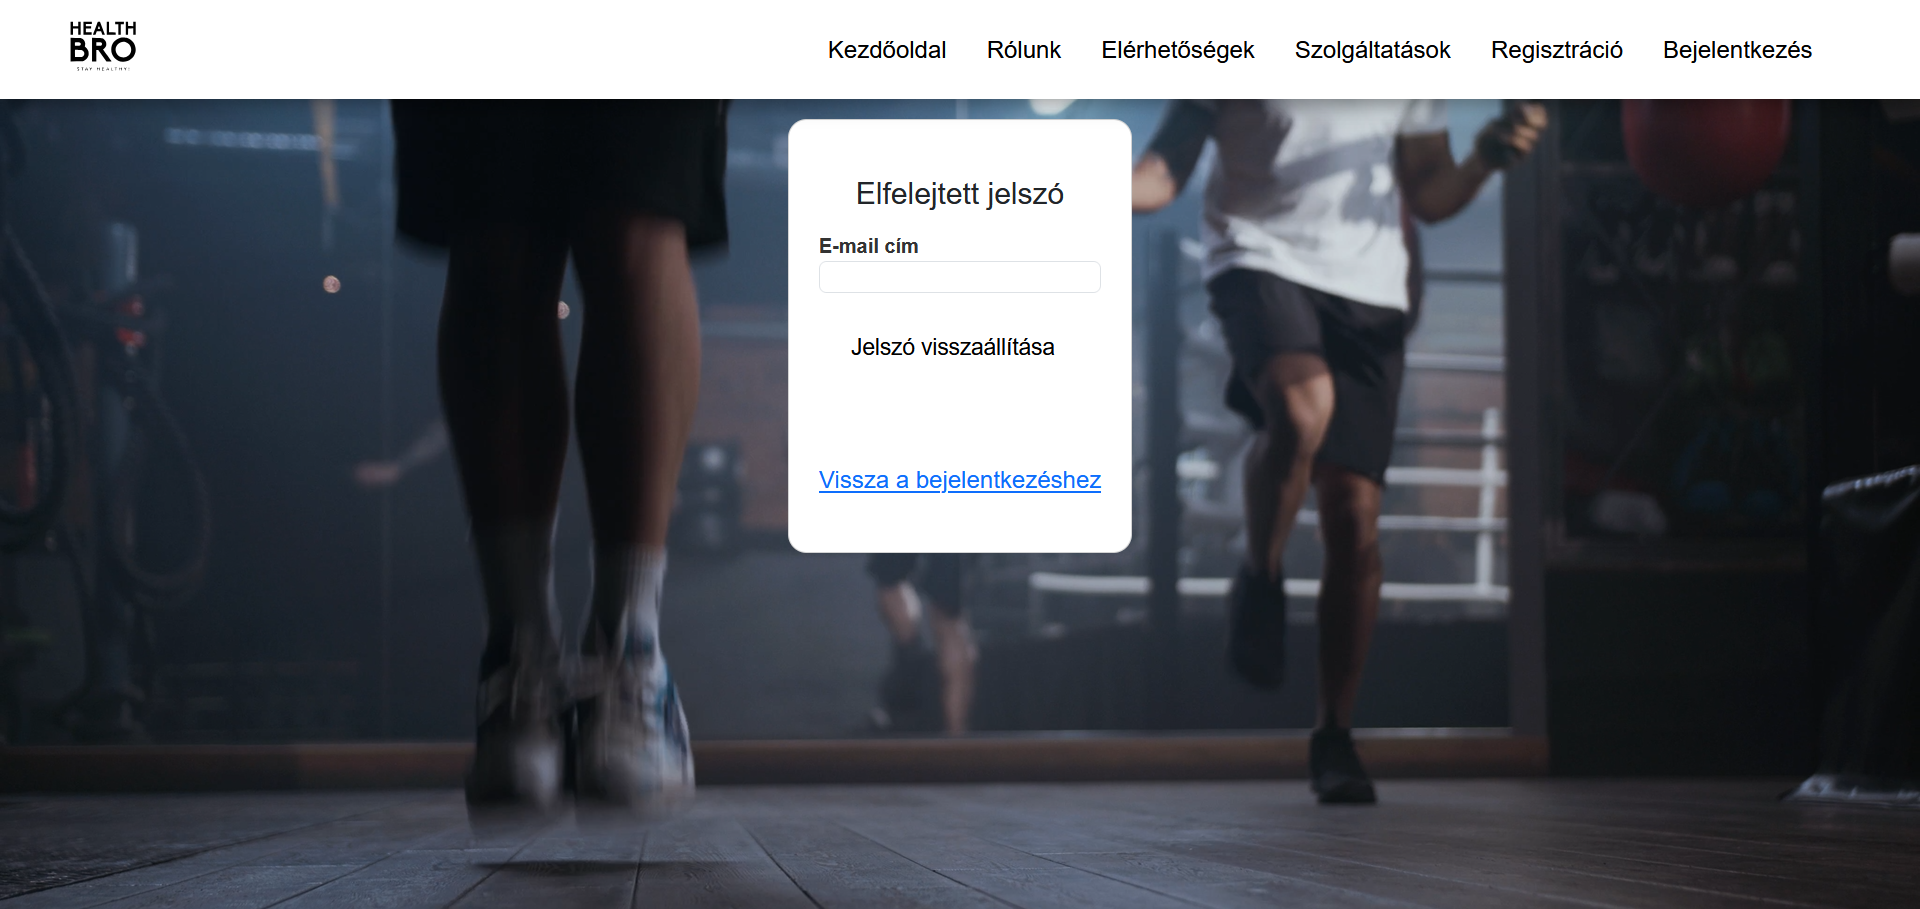
\includegraphics[width=1\textwidth]{figures/elfelejtettpw.png}\\[0.5cm]}

\section{Funkciók részletes bemutatása}
\subsection{Alapfunkciók}
\begin{itemize}
	\item \textbf{Edzésnapló hozzáadása}: Minden edzés után rögzítheted az elvégzett gyakorlatokat, ismétléseket, súlyokat.
	\item \textbf{Edzésprogramok választása}: Különböző edzésprogramok elérhetők a felhasználók számára.
\end{itemize}

\chapter{Hibaelhárítás és támogatás}
\section{Gyakori problémák}
\textbf{Probléma}: Az oldal nem tölt be megfelelően.\\
\textbf{Megoldás}: Ellenőrizd az internetkapcsolatot és próbáld meg frissíteni az oldalt.

\section{Kapcsolatfelvétel támogatásért}
Ha további segítségre van szükséged:
\begin{itemize}
	\item E-mail: \href{mailto:support@healthbro.com}{support@healthbro.com}
	\item Telefon: +36 1 234 5678
\end{itemize}

\chapter{Mellékletek}
\section{GYIK}
\begin{itemize}
	\item Hogyan tudok regisztrálni?
	\item Miért nem tudok ékezetes karaktereket megadni jelszónak?
	\item Hogyan hozhatok létre edzéstervet?
	\item Hogyan módosíthatom a metrikus beállításokat?
	
\end{itemize}

\section{További források}
\begin{itemize}
	\item \href{https://www.fitnessalapok.com}{Fitness alapok – Weboldal}
	\item \href{https://www.healthbro.com/blog}{Edzésprogramok – Blog}
\end{itemize}

\chapter*{Összegzés}
\addcontentsline{toc}{chapter}{Összegzés}
A HealthBro egy webalapú edzéskövető alkalmazás, amely lehetőséget biztosít a felhasználóknak edzésprogramjaik dokumentálására és fejlődésük nyomon követésére. Az alkalmazás célja, hogy a felhasználók könnyen rögzíthessék edzéseiket, beállíthassák céljaikat, és statisztikai eszközökkel figyelemmel kísérhessék fejlődésüket. A rendszer tartalmazza az edzések naplózásának, célok beállításának és haladás nyomon követésének funkcióit. Az alkalmazás felhasználóbarát felületet biztosít, amely böngészőkön keresztül elérhető, így nincs szükség telepítésre. A felhasználói élmény további javítása érdekében reszponzív dizájnt alkalmazunk, így az oldal minden eszközön optimálisan működik. A regisztráció és bejelentkezés folyamata egyszerű, és lehetővé teszi, hogy bárki könnyedén hozzáférjen a funkciókhoz. Az alkalmazásban a csapatunk folyamatosan dolgozik a fejlesztésen, és jövőbeli terveink között szerepel a mobilalkalmazás verziója is. Az eszközök és funkciók folyamatosan fejlődnek, hogy a felhasználók számára a legjobb élményt biztosítsák. A dokumentáció célja, hogy részletes információkat adjon az alkalmazás használatáról és segítse a felhasználókat a rendszer megértésében.

\newpage
\Huge\begin{center}
	\textbf{Köszönetnyilvánítás}	
\end{center}\normalsize
Szeretném kifejezni hálámat és köszönetemet azoknak, akik hozzájárultak tudásom és fejlődésem megszerzéséhez. Különösen hálás vagyok:
\newline
\newline
Németh Bence, az IKT projekmenedzsment és frontend oktatója, aki értékes tanácsaival és szakmai iránymutatásaival segítette a projekt sikeres megvalósítását.
\newline
Kerényi Róbert Nándor, a backend oktatója, aki mélyreható ismeretekkel és türelemmel segítette az összetett backend problémák megértését.
\newline
Deák Csaba, az asztali és mobilalkalmazás oktatója, aki hozzájárult a projekt alkalmazásainak fejlesztéséhez, valamint a mobil platformokon való működtetéshez.
\newline
Takács István, az adatbázis oktatója, akinek iránymutatásai nélkül nem lett volna lehetséges az adatok kezelésének hatékony megoldása.
\newline
\newline
Köszönöm mindannyiuknak a folyamatos támogatást és inspirációt!



\begin{thebibliography}{2}
\addcontentsline{toc}{chapter}{\bibname}
\bibitem{VartereszI1} \textsc{Várterész Magdolna}: \emph{Az informatika logika alapjai előadások}, 2006/07-es tanév 1.félév, \url{http://users.atw.hu/de-mi/index.php?r=file/download\&id=219},  Letöltve: 2019 március 12.-én 

\bibitem{internet} \textsc{Forrás}: 
\emph{Ezen a napon (2024.10.22) ez alapján a forrás alapján írtuk meg a dokumentációmat}, Szakmai vizsga, \url{http://netpedia.hu/relacios-adatbazis}
\end{thebibliography}

% Ide lehet szkennelt dokumentumot, dokumentumokat beszúrni
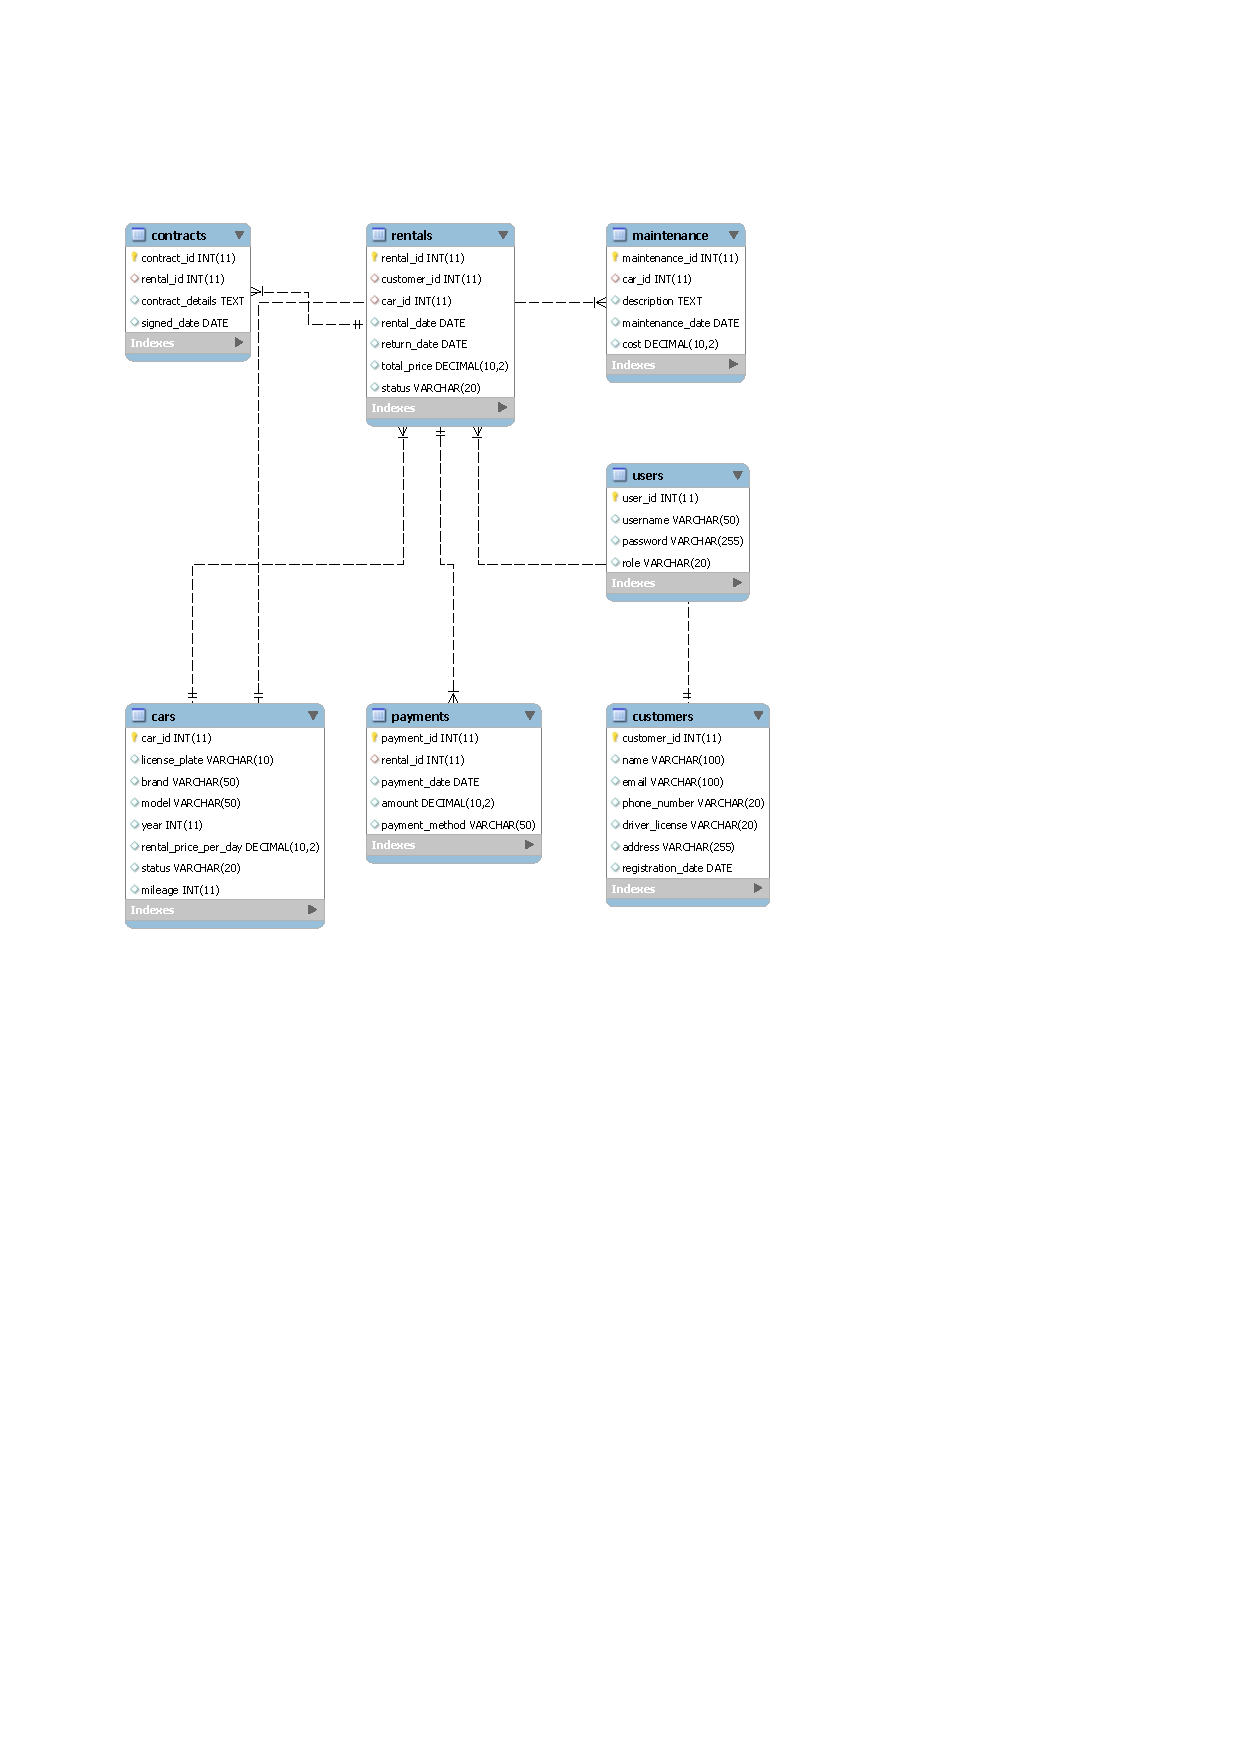
\includepdf{figures/td.pdf}


\end{document}